\documentclass[10pt,a4paper]{article}
\usepackage[margin=17mm]{geometry}
\usepackage{graphicx,booktabs,hyperref}
\pagestyle{empty}
\begin{document}
\noindent{\Large\bfseries Current scan worker: control qualification}\\[3pt]
{\small Rust, 27 November 2026. PR \#5251. No measured runtime result.}\\[3pt]
{\small $p=2147483647,9007199254740881$; $n=3,4,6$; seed7 LAST-star.}
\paragraph{Result.} The rebuilt current-root worker completes all 432 no-clock transport calls, with 432 complete parent proof replays and 1728 deliberate corruptions rejected. All 45 unit functions pass: worker2, transport9, collector9, analyzer16, fixture9. These are unsigned same-host checks. No actual comparative observation is collected. [pcc:unverified]
\begin{center}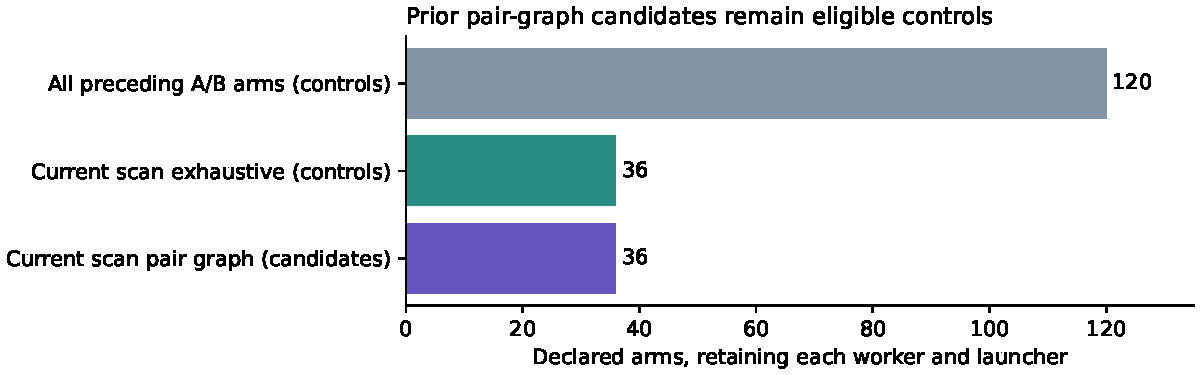
\includegraphics[width=\linewidth]{control-roster.pdf}\end{center}
\noindent All 120 preceding A/B arms remain eligible controls, including earlier root pair-graph candidates, with their exact worker, kind, kernel and launcher. Adding 36 current scan-exhaustive controls gives 156 controls for 36 current scan-pair-graph candidates. The fixed primary is scan-root-pairgraph-flat-dag-487-native. There are 312 A/A arms, 192 A/B arms, five rounds and six inputs: 15120 future calls, none measured.
\paragraph{Synthetic checks.} Two explicitly synthetic cohorts each complete 15120 full proof replays. The neutral cohort chooses the earlier root pair-graph control in every case/round and rejects threshold arithmetic. The hypothetical20 cohort clears arithmetic. Admission remains false for both. All clocks and monitor flags are invented; none is an observed host runtime, contention state or A/A measurement. [pcc:unverified]
\begin{center}\begin{tabular}{lrrr}\toprule
Synthetic scenario & Whole proofs & Arithmetic passes & Admission\\\midrule
Neutral &15120 &false &false\\
Hypothetical20 &15120 &true &false\\\bottomrule
\end{tabular}\end{center}
\noindent Copied clock-receipt and duplicate-cell sabotage views are refused without an analysis report. Every neutral source-file digest remains unchanged. Qualification worker phases remain null; parent replay checks every full original proof, native basis, statistics and receipt binding. [pcc:unverified]
\newpage
\noindent{\Large\bfseries Boundary, provenance and remaining acceptance}
\paragraph{Full call retained.} Parent command/raw capture and capped child launch; input read/decoding; complete root API construction, wire replay and native certification; additional worker proof readback; proof writes/transport; process receipt; complete parent replay and basis/statistics/hash binding all remain inside the agreed application call. Root setup is not amortized. Case-directory creation and final outcome/report writes remain outside the original frozen boundary. Diagnostic phases cannot substitute for the whole call.
\paragraph{Source.} SOURCE\_V2 adds this instrument to the canonical-scan production context; no production source changes here. Root-worker source is byte-identical to the previous instrument but rebuilt against the current actual library. Historical rosters and evidence remain unchanged. Every registry dependency version/checksum matches the previous lock. PRECALL pins five comparison workers and ten immutable instrument/libtest tools.
\paragraph{Retained corrections.} Initial normal/unit builds succeed. Static inspection, before qualification, catches inconsistent proposed synthetic parent400/child300/worker400. V2 uses parent500/child400/worker400. Initial source and build logs remain; V2 reused source-pre/postcheck log paths, so separate V1 source-check logs are not claimed. A nonexistent metadata corpus path is corrected and all six input hashes checked before calls. An inherited canary output prefix is refused before mutation and corrected in a separate runner. Sparse helper-script omissions are preserved as setup errors; helpers are restored byte-exactly. Sparse lessons output does not establish absence of lessons. No numerical rerun hides a failed cohort.
\paragraph{Scope and custody.} Rust1.100.0, opt0/LTOoff/debug0/incrementalfalse/codegen16, default-features=false, CPU0/jobs1 and one numerical thread are correctness settings, not optimized performance qualification. Complete current transport, both synthetic cohorts, both copied sabotage/refusal views and ten frozen tools are archived with complete member-byte checks. Prior full-root libtest allocation failures remain separate. The B5 CI snapshot has successful native checks and a failed artifact migration; it is not an all-workflow pass. Intrinsic regularity and actual F4 solving degree remain unknown.
\paragraph{Sources reviewed.} Prior four-worker collector/analyzer/fixture/rosters, native supervisor, draft372 and the current production scan/parity qualification. KB tools/wrapper are unavailable in this runtime; no novelty claim is made. Figure rendering only lays out recorded configuration/results.
\paragraph{Next acceptance.} Original 15$\times$ acceptance still needs prospectively pinned repeated full-call measurements against strongest matched controls, A/A, all six fixed cases, all proofs/failures and published validated evidence. Conductor and checkpoint/S3 access are waived. The separate required canonical timing document remains encrypted; the existing document-only choice is unanswered. Collector rejects unqualified or synthetic pins; draft analyzer admission stays false. This study grants no timing authorization, cost-model credit or 15$\times$ result. No key, gate, ledger or original test is weakened.
\end{document}
